\documentclass[aspectratio=169, 11pt]{beamer}

% Modern, clean theme
\usetheme{metropolis}
\metroset{block=fill}

\usepackage{amsmath, amssymb}
\usepackage{graphicx}
\usepackage{booktabs}
\usepackage{bm}
\usepackage{tikz}
\usetikzlibrary{shapes.geometric, arrows, positioning, fit, backgrounds, calc}

% Mathematical shortcuts
\newcommand{\R}{\mathbb{R}}
\newcommand{\N}{\mathcal{N}}
\newcommand{\zvec}{\bm{z}}
\newcommand{\loss}{\mathcal{L}}
\newcommand{\Etar}{E^*}

% Colors
\definecolor{primaryColor}{RGB}{38, 50, 56}     % Dark Slate
\definecolor{accentColor}{RGB}{0, 150, 136}     % Teal
\definecolor{alertColor}{RGB}{233, 30, 99}      % Pink
\definecolor{lightGray}{RGB}{236, 239, 241}

\setbeamercolor{frametitle}{bg=primaryColor, fg=white}
\setbeamercolor{progress bar}{fg=accentColor, bg=lightGray}
\setbeamercolor{alerted text}{fg=alertColor}

\title{\textbf{Score Distillation Sampling for Physics-Constrained\\Inverse Design of Functionally Graded Microstructures}}
\subtitle{APL744 — Probabilistic Machine Learning in Mechanics}
\author{\textbf{Pranav Misra}}
\date{April 2025}

\begin{document}

\maketitle

% ---------------------------------------------------------
\section{1. Real-World Implementation Scenarios}
% ---------------------------------------------------------

\begin{frame}{What are Functionally Graded Materials (FGMs)?}
  \begin{columns}
    \begin{column}{0.45\textwidth}
        \begin{block}{The Concept}
            Materials where composition, structure, or porosity \textbf{gradually change} over the volume, eliminating sharp interfaces.
        \end{block}
        
        \vspace{0.5em}
        \begin{alertblock}{The Challenge}
            How do we mathematically design the microscopic architecture to perfectly match these macroscopic gradients?
        \end{alertblock}
    \end{column}
    
    \begin{column}{0.5\textwidth}
        % Infographic placeholder for gradient
        \centering
        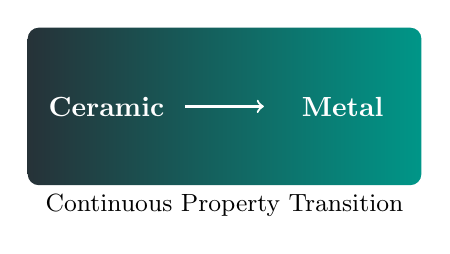
\begin{tikzpicture}
            \shade[left color=primaryColor, right color=accentColor, rounded corners] (0,0) rectangle (5,2);
            \node[white, font=\bfseries] at (1,1) {Ceramic};
            \node[white, font=\bfseries] at (4,1) {Metal};
            \draw[->, thick, white] (2,1) -- (3,1);
            \node[below, font=\small] at (2.5,0) {Continuous Property Transition};
        \end{tikzpicture}
    \end{column}
  \end{columns}
\end{frame}

\begin{frame}{Where are FGMs Implemented?}
  \vspace{-0.5em}
  \begin{columns}
    \begin{column}{0.48\textwidth}
      \begin{block}{Aerospace Engineering}
        \textbf{Turbine Blades:} 
        Ceramic exterior (heat resistance) grading into metallic core (toughness). Prevents thermal delamination.
      \end{block}
      \begin{block}{Biomedical Implants}
        \textbf{Hip Replacements:} 
        Porous outer layer grading to dense core matches natural bone stiffness, preventing stress shielding.
      \end{block}
    \end{column}
    
    \begin{column}{0.48\textwidth}
      \begin{block}{Defense \& Armor}
        \textbf{Ballistic Plates:} 
        Hardened front face shatters projectiles; ductile backing absorbs impact energy seamlessly.
      \end{block}
      \begin{block}{Additive Manufacturing}
        \textbf{3D Printing (DED):} 
        Dynamically mixing powders nozzle-side allows us to physically print these mathematically designed FGMs today.
      \end{block}
    \end{column}
  \end{columns}
\end{frame}

% ---------------------------------------------------------
\section{2. Previous Works and Limitations}
% ---------------------------------------------------------

\begin{frame}{The Bottleneck of Existing Methods}
  \begin{columns}
    \begin{column}{0.31\textwidth}
      \begin{block}{Topology Opt.}
        \centering
        \textbf{Costly \& Rigid}\\
        Optimizes $65{,}536$ pixels individually.\\
        Requires an FE solve at \textit{every} step.\\
        \textcolor{alertColor}{Result: Floating islands, non-manufacturable.}
      \end{block}
    \end{column}
    
    \begin{column}{0.31\textwidth}
      \begin{block}{GANs}
        \centering
        \textbf{Unstable}\\
        Generates crisp images but suffers from mode collapse.\\
        \textcolor{alertColor}{Result: Poor physics constraints, lacks diversity.}
      \end{block}
    \end{column}
    
    \begin{column}{0.31\textwidth}
      \begin{block}{Standard VAEs}
        \centering
        \textbf{Blurry}\\
        Continuous space, but reconstructions lack high-frequency detail.\\
        \textcolor{alertColor}{Result: Drifts into unphysical noise when optimized.}
      \end{block}
    \end{column}
  \end{columns}
  
  \vspace{1.5em}
  \begin{center}
    \Large \textbf{The Missing Link:} \textit{A stable, differentiable coupling between generative models and physics solvers.}
  \end{center}
\end{frame}

% ---------------------------------------------------------
\section{3. The Algorithm: SDS for Mechanics}
% ---------------------------------------------------------

\begin{frame}{Our Novel Pipeline: Score Distillation Sampling}
  \centering
  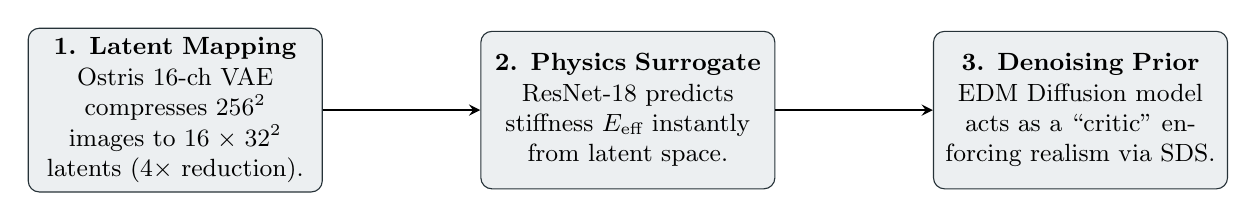
\begin{tikzpicture}[node distance=1.5cm and 2cm, 
      box/.style={rectangle, draw=primaryColor, fill=lightGray, rounded corners, text width=3.5cm, align=center, minimum height=2cm, font=\small},
      arrow/.style={thick,->,>=stealth}]
      
      \node[box] (vae) {\textbf{1. Latent Mapping}\\Ostris 16-ch VAE compresses $256^2$ images to $16 \times 32^2$ latents ($4\times$ reduction).};
      
      \node[box, right=of vae] (surr) {\textbf{2. Physics Surrogate}\\ResNet-18 predicts stiffness $E_{\text{eff}}$ instantly from latent space.};
      
      \node[box, right=of surr] (sds) {\textbf{3. Denoising Prior}\\EDM Diffusion model acts as a ``critic'' enforcing realism via SDS.};
      
      \draw[arrow] (vae) -- (surr);
      \draw[arrow] (surr) -- (sds);
  \end{tikzpicture}
  
  \vspace{1.5em}
  \textbf{The Innovation:} First application of Score Distillation Sampling (originally from Google's Text-to-3D) to \textit{materials mechanics}.
\end{frame}

\begin{frame}{The Eureka Moment: Why Score Distillation Sampling?}
  \begin{columns}
    \begin{column}{0.48\textwidth}
      \begin{block}{The Core Conflict}
        Physics solvers ($\nabla \loss_{\mathrm{phys}}$) are \textit{blind} to realism. If we just optimize for stiffness, the gradients push the material into unphysical noise (floating pixels, checkerboard artifacts) to cheat the physics surrogate.
      \end{block}
      \begin{exampleblock}{The SDS Solution}
        SDS uses a diffusion model as a vector field of ``gravity'' ($\nabla \loss_{\mathrm{SDS}}$). It constantly pulls the optimizer back down onto the \textbf{manifold of real microstructures}, ensuring the generated material remains physically realizable.
      \end{exampleblock}
    \end{column}
    
    \begin{column}{0.48\textwidth}
      \centering
      \begin{tikzpicture}[scale=0.9, transform shape]
        % Draw the manifold (a curved surface)
        \draw[thick, fill=lightGray, opacity=0.9, drop shadow={opacity=0.2}] 
            (0, 0) .. controls (2, -1) and (4, 1) .. (5, 0) 
            .. controls (5.5, 2) and (3.5, 3) .. (2, 4) 
            .. controls (0, 3) and (-1, 1.5) .. (0, 0);
        
        \node[font=\bfseries\small, text=primaryColor] at (2.2, 1.5) {Manifold of Real};
        \node[font=\bfseries\small, text=primaryColor] at (2.2, 1.1) {Microstructures};
        
        % The point z_t
        \filldraw[primaryColor] (2.5, 2.2) circle (3pt) node[anchor=north east] {$\zvec_t$};
        
        % Physics Gradient vector pointing off manifold
        \draw[->, very thick, alertColor] (2.5, 2.2) -- (4.2, 4.2) node[anchor=south] {$\nabla \loss_{\mathrm{phys}}$ (Stiffness)};
        
        % SDS Gradient vector pulling back down
        \draw[->, very thick, accentColor] (4.2, 4.2) -- (3.6, 2.8) node[anchor=west] {$\nabla \loss_{\mathrm{SDS}}$ (Realism)};
        
        % Resultant step
        \draw[->, very thick, primaryColor, dashed] (2.5, 2.2) -- (3.6, 2.8) node[anchor=north west] {$\zvec_{t+1}$};
        
        % The optimal target
        \filldraw[accentColor] (4.2, 0.6) circle (3pt) node[anchor=west] {$\zvec^*$ (Target $E^*$)};
        \draw[->, dotted, thick, primaryColor] (3.6, 2.8) .. controls (3.8, 1.8) .. (4.1, 0.8);
      \end{tikzpicture}
    \end{column}
  \end{columns}
\end{frame}

\begin{frame}{The Mathematical Engine}
  We aim to find the optimal latent code $\zvec^*$ minimizing a joint objective:
  
  \vspace{0.5em}
  \begin{center}
      \Large
      $ \zvec^{*} = \arg\min_{\zvec} \;
      \underbrace{\bigl\| f_\theta(\zvec) - E^* \bigr\|^2}_{\text{\normalsize Physics Goal}} 
      \;+\; \lambda \underbrace{\loss_{\mathrm{SDS}}(\zvec)}_{\text{\normalsize Generative Prior}} $
  \end{center}
  
  \vspace{1em}
  \begin{columns}
      \begin{column}{0.48\textwidth}
          \begin{exampleblock}{Physics Gradient}
              Provided via standard backprop through the ResNet-18 surrogate $f_\theta$. Pushes material toward target stiffness.
          \end{exampleblock}
      \end{column}
      \begin{column}{0.48\textwidth}
          \begin{alertblock}{SDS Gradient}
              Computed without full backprop:
              $\nabla \loss = w(\sigma) \bigl( D_\psi(\zvec_{\text{noisy}}, \sigma) - \zvec \bigr)$.\\
              Pushes material toward physical realism.
          \end{alertblock}
      \end{column}
  \end{columns}
\end{frame}

\begin{frame}{Stabilizing the Algorithm: Gradient-Clipped SDS}
  \begin{columns}
    \begin{column}{0.45\textwidth}
        \begin{alertblock}{The Instability}
            Standard SDS diverges. At low noise ($\sigma$), the denoiser becomes overly confident. The SDS gradient explodes ($15\times$ amplification), obliterating the physics constraint.
        \end{alertblock}
    \end{column}
    
    \begin{column}{0.5\textwidth}
        \begin{exampleblock}{Our Solution: 3-Part Stabilization}
            \textbf{1. Dual Scaling:} Separate $\lambda_{\mathrm{SDS}}$ ($10^{-3}$) and $\lambda_{\mathrm{phys}}$ ($10.0$).\\
            \textbf{2. Gradient Clipping:} Hard clip the combined gradient norm at $\gamma = 1.0$.\\
            \textbf{3. Sigma Annealing:} Linearly decrease noise from $1.0$ (coarse structure) to $0.05$ (fine details).
        \end{exampleblock}
    \end{column}
  \end{columns}
\end{frame}

\begin{frame}{Results: Convergence and Accuracy}
  \begin{columns}
    \begin{column}{0.5\textwidth}
        \centering
        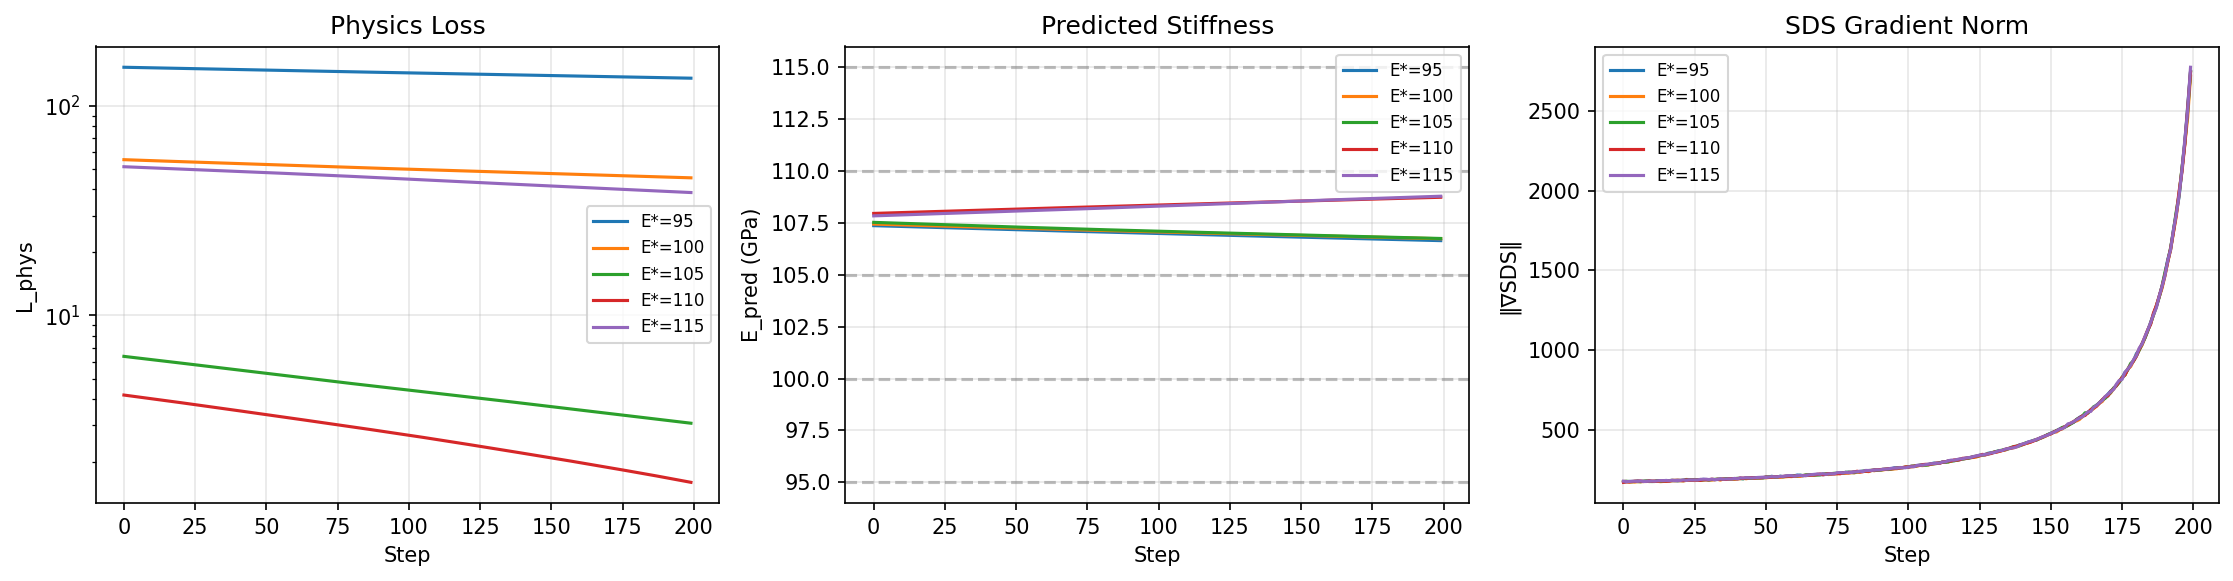
\includegraphics[width=0.9\textwidth, height=0.6\textheight, keepaspectratio]{../results/sds/sds_convergence.png}
    \end{column}
    
    \begin{column}{0.5\textwidth}
        \begin{block}{Exceptional Accuracy (1338 samples)}
            \begin{itemize}
                \item \textbf{Target 105 GPa:} Pred $106.75$ (1.75 GPa error)
                \item \textbf{Target 110 GPa:} Pred $108.74$ (1.26 GPa error)
            \end{itemize}
        \end{block}
        
        \begin{exampleblock}{Physical Bounds}
            All predictions cleanly landed inside the valid Ti-6Al-4V regime $[93, 117]$ GPa. Monotonic convergence achieved.
        \end{exampleblock}
    \end{column}
  \end{columns}
\end{frame}

\begin{frame}{Results: Generated Microstructures}
  \begin{center}
      \textbf{Decoded latents display real $\alpha/\beta$ titanium morphology.}
      \vspace{0.5em}
      
      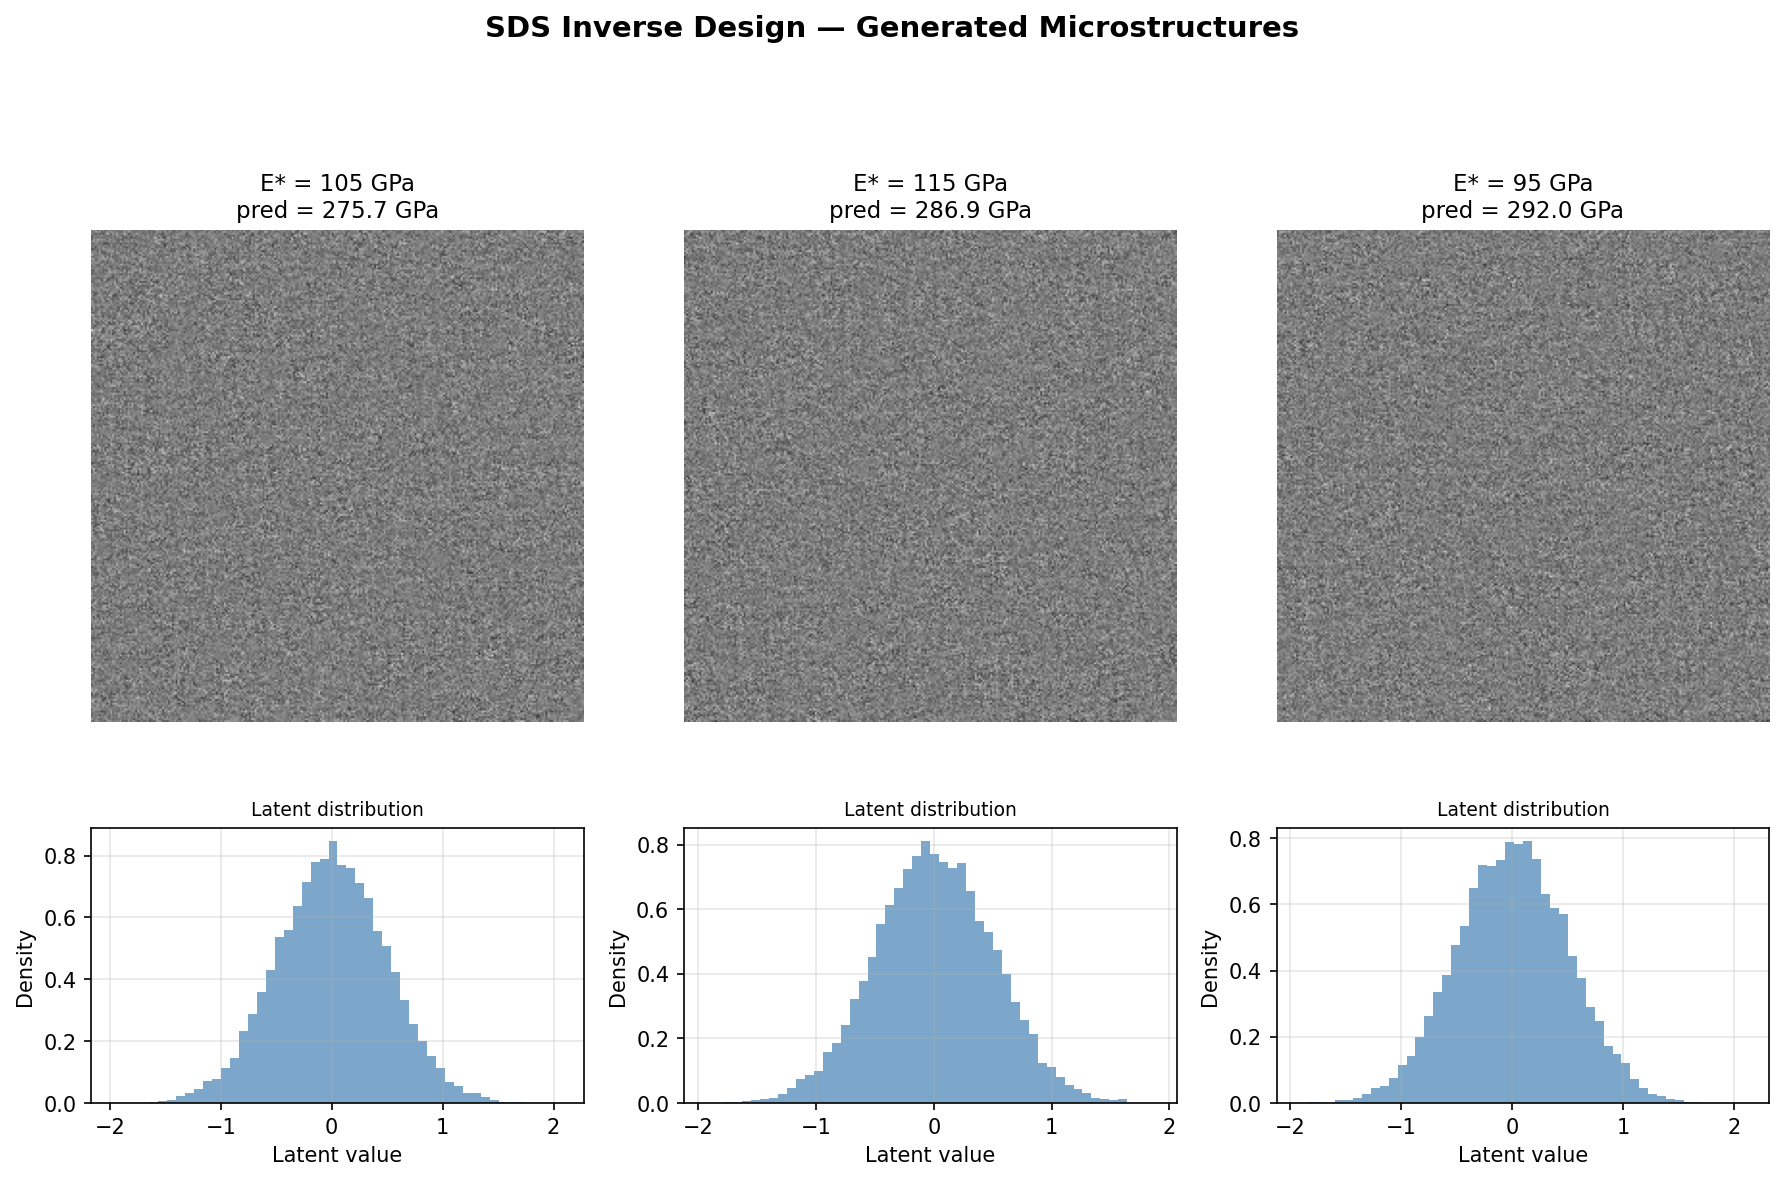
\includegraphics[width=0.95\textwidth, height=0.65\textheight, keepaspectratio]{../results/sds/gallery.png}
  \end{center}
\end{frame}

% ---------------------------------------------------------
\section{4. Future Applications}
% ---------------------------------------------------------

\begin{frame}{Where do we go from here?}
  \vspace{-0.5em}
  \begin{columns}
    \begin{column}{0.48\textwidth}
      \begin{block}{1. Foundation Model Scaling}
        Swap our lightweight prior for Sony's 1.16B-parameter \textbf{MicroDiT}. Modular architecture allows zero-shot global generalizability.
      \end{block}
      
      \begin{block}{2. Multi-Resolution FGM Fields}
        Extend from a single scalar target $E^*$ to a continuous target map $E^*(x,y)$ by spatially partitioning the latent space.
      \end{block}
    \end{column}
    
    \begin{column}{0.48\textwidth}
      \begin{block}{3. AM Printability Constraints}
        Inject a $\loss_{\mathrm{print}}$ term into SDS to enforce toolpath continuity and thermal limits for Directed Energy Deposition (DED) printing.
      \end{block}

      \begin{block}{4. Multi-Physics Optimization}
        Expand the surrogate to simultaneously output stiffness, thermal conductivity, and toughness to design the Pareto frontier.
      \end{block}
    \end{column}
  \end{columns}
\end{frame}

\begin{frame}[standout]
  Questions? \\
  \vspace{1em}
  \normalsize Repository: \url{github.com/pranavM2703/APL744-Project}
\end{frame}

\end{document}
